% !TeX spellcheck = es_AR
\documentclass[12pt,a4paper]{article}

%Packages

%%% Geometria y fuente %%%
\usepackage[utf8]{inputenc}
\usepackage[spanish,es-noquoting]{babel}
\usepackage{geometry}
\geometry{a4paper,left=20mm,right=20mm,top=20mm,bottom=20mm}
\usepackage{bookman} % font
\usepackage{authblk} % estilo de titulo, autor y afiliación
\renewcommand*{\Authfont}{\small\itshape}
\renewcommand*{\Affilfont}{\small\itshape}
\usepackage{setspace} % para modificar el interlineado
%\setlength\parindent{0pt}  elimina sangría de todos los parrafos


%%% Mathematical tools %%%
\usepackage{marvosym}
\usepackage{amsmath}
\usepackage{mathrsfs}
\usepackage{mathtools}
\numberwithin{equation}{section}
\usepackage{amssymb}
\usepackage{bm}


%%% Box and colors %%%
\usepackage{color}
\usepackage{tcolorbox}
\newtcolorbox{boxumen}{colback=white,colframe=teal,boxrule=1pt}
\newtcolorbox{boxquation}{colback=white,colframe=black,boxrule=1pt}


%%% Capital Letter %%%
\usepackage{lettrine} % letra capital}
\setcounter{DefaultLines}{4}
\setlength{\DefaultFindent}{7pt}
\setlength{\DefaultNindent}{0pt}
\renewcommand{\LettrineFontHook}{\usefont{U}{yinit}{m}{n}}
\renewcommand{\DefaultLoversize}{-0.70}
\usepackage{yfonts}
%Primero se declara el paquete lettrine y el numero de renglones que debe abarcar la inicial. En seguida DefaultFindent, la distancia de la inicial a la letra siguiente en el primer renglón y DefaultNindent, la distancia que se desplaza a la derecha del inicio del primer renglón, los renglones subsecuentes que abarca la capitular.Después se declara la font a utilizar, en este caso yinit, con unos parámetros que la describen, y finalmente el tamaño de la letra.


%%% Pagestyle %%%
\usepackage{fancyhdr}

\fancypagestyle{lab}{
\fancyhf{}
\rhead{{\color{brown!60!black}\Large\Coffeecup}}
\lhead{\textit{\small{Laboratorio 6}}}
\fancyfoot{}
%\lfoot{\tiny{}}
\rfoot{\thepage}
}
\fancypagestyle{informe}{
	\fancyhf{}
	\rhead{{\color{brown!60!black}\Large\Coffeecup}}
	\lhead{\textit{\small{Informe de Avance}}}
	\fancyfoot{}
	%\lfoot{\tiny{}}
	\rfoot{\thepage}
}


%Hace títulos pequeños
\usepackage[tiny]{titlesec}
%es pa que la intro quede en 1pag con abstract de 5 renglones


\title{\vspace{-40pt}\Large{\textbf{\textcolor{teal}{Construcción de detectores de muones con centellador plástico para la caracterización de detectores de partículas por Cherenkov en agua}}}}

\date{}

\author{\vspace{-.3cm}Barboza, Gastón; Codina, Tomás} 
\affil{\vspace{-.3cm}Instituto de Astronomía y Física del Espacio}
\affil{\vspace{-.3cm}Laboratorio 6, Departamento de Física, FCEyN, UBA}
\affil{\vspace{-.3cm}barboza.gaston@gmail.com, tomycodina@gmail.com\vspace{.2cm}}




%Document
\begin{document}


\maketitle
\thispagestyle{lab}

\begin{center}
\vspace{-40pt}\rule{\textwidth}{0.2pt}
\end{center}

\setstretch{1.5} % Interlineado 1.5
\small
\begin{boxumen}
Se caracterizó la señal emitida por dos barras centelladoras relevada con fotomultiplicadores, tanto de manera individual como en coincidencia, con el objetivo de detectar el paso de muones. Para ello, se construyó un entorno oscuro adecuado para el funcionamiento del instrumental y se relevaron los datos a través de osciloscopio. Se verificó la existencia de una señal independiente del ruido del sistema correspondiente a la detección de estas partículas, y se estableció un valor tentativo para la eficiencia del detector.
\end{boxumen}
\normalsize
\section{Introducción}

Los rayos cósmicos llegan a la tierra desde todas direcciones del espacio con energías que van desde alrededor de 1 GeV hasta cientos
de EeV ($10^{18}$eV). Los detectores de rayos cósmicos son utilizados por muchos experimentos que necesitan observar estos rayos con distintos propósitos; por ejemplo el Observatorio LAGO los utiliza para el estudio de la actividad solar, o el Observatorio Pierre Auger para investigar el origen de los rayos cósmicos ultraenergéticos.

Este tipo de observatorios pueden utilizar uno o muchos detectores individuales, cuyas características deben ser estudiadas para determinar sus condiciones de diseño. Para este tipo de desarrollo se utilizan detectores auxiliares que identifican la trayectoria y naturaleza de alguna partícula que entra al detector, lo cual permite estudiar el tipo de señal que este genera. Un tipo particular de detector auxiliar de reducidas dimensiones es el comúnmente llamado ``paleta centelladora''. Consta de un centellador plástico con un detector óptico adosado; este registra los pulsos de luz que se producen en el centellador al ser atravesado por una partícula cargada. 

El objetivo del trabajo a realizar en laboratorio 6 consiste en construir y caracterizar los componentes básicos de estas paletas centelladoras.

\section{Montaje Experimental y Adquisición}

Se utilizó la tecnología del detector AMIGA del Observatorio Pierre Auger\cite{pierreauger}, cuyo elemento básico consta de una barra centelladora recorrida en su longitud por fibras ópticas. Estas colectan la luz producida por el centellador y la guían
hacia un tubo fotomultiplicador (o PMT, por sus siglas en inglés). Se armaron dos detectores para medir eventos simultáneos o ``coincidencias'', para filtrar los pulsos de ruido de aquellos producidos por muones.

Dada la sensibilidad del PMT, se construyó un entorno a prueba de luz para realizar las mediciones. Se recubrió una caja de madera de $ 92\times42\times20\text{cm}^3$ con aluminio, con dos perforaciones para el ingreso de cables. Una perforación fue sellada con un conector para la alimentación, con una luz testigo externa para indicar el cierre del circuito. A la otra perforación se le colocó una conexión de tanque de PVC, en forma de U para evitar el ingreso de luz; a través de ella salían los cables de señal de los PMT. La holgura de la tapa fue rellenada con felpa negra, el interior de la caja fue pintado de negro para evitar rebotes, y finalmente se utilizó tela \textit{blackout} para cubrir la caja durante su uso. Como medida de seguridad para evitar dañar los PMT, se colocaron micro switch debajo de la tapa para interrumpir la alimentación si fuese levantada. 

\begin{figure}[h]
	\centering
	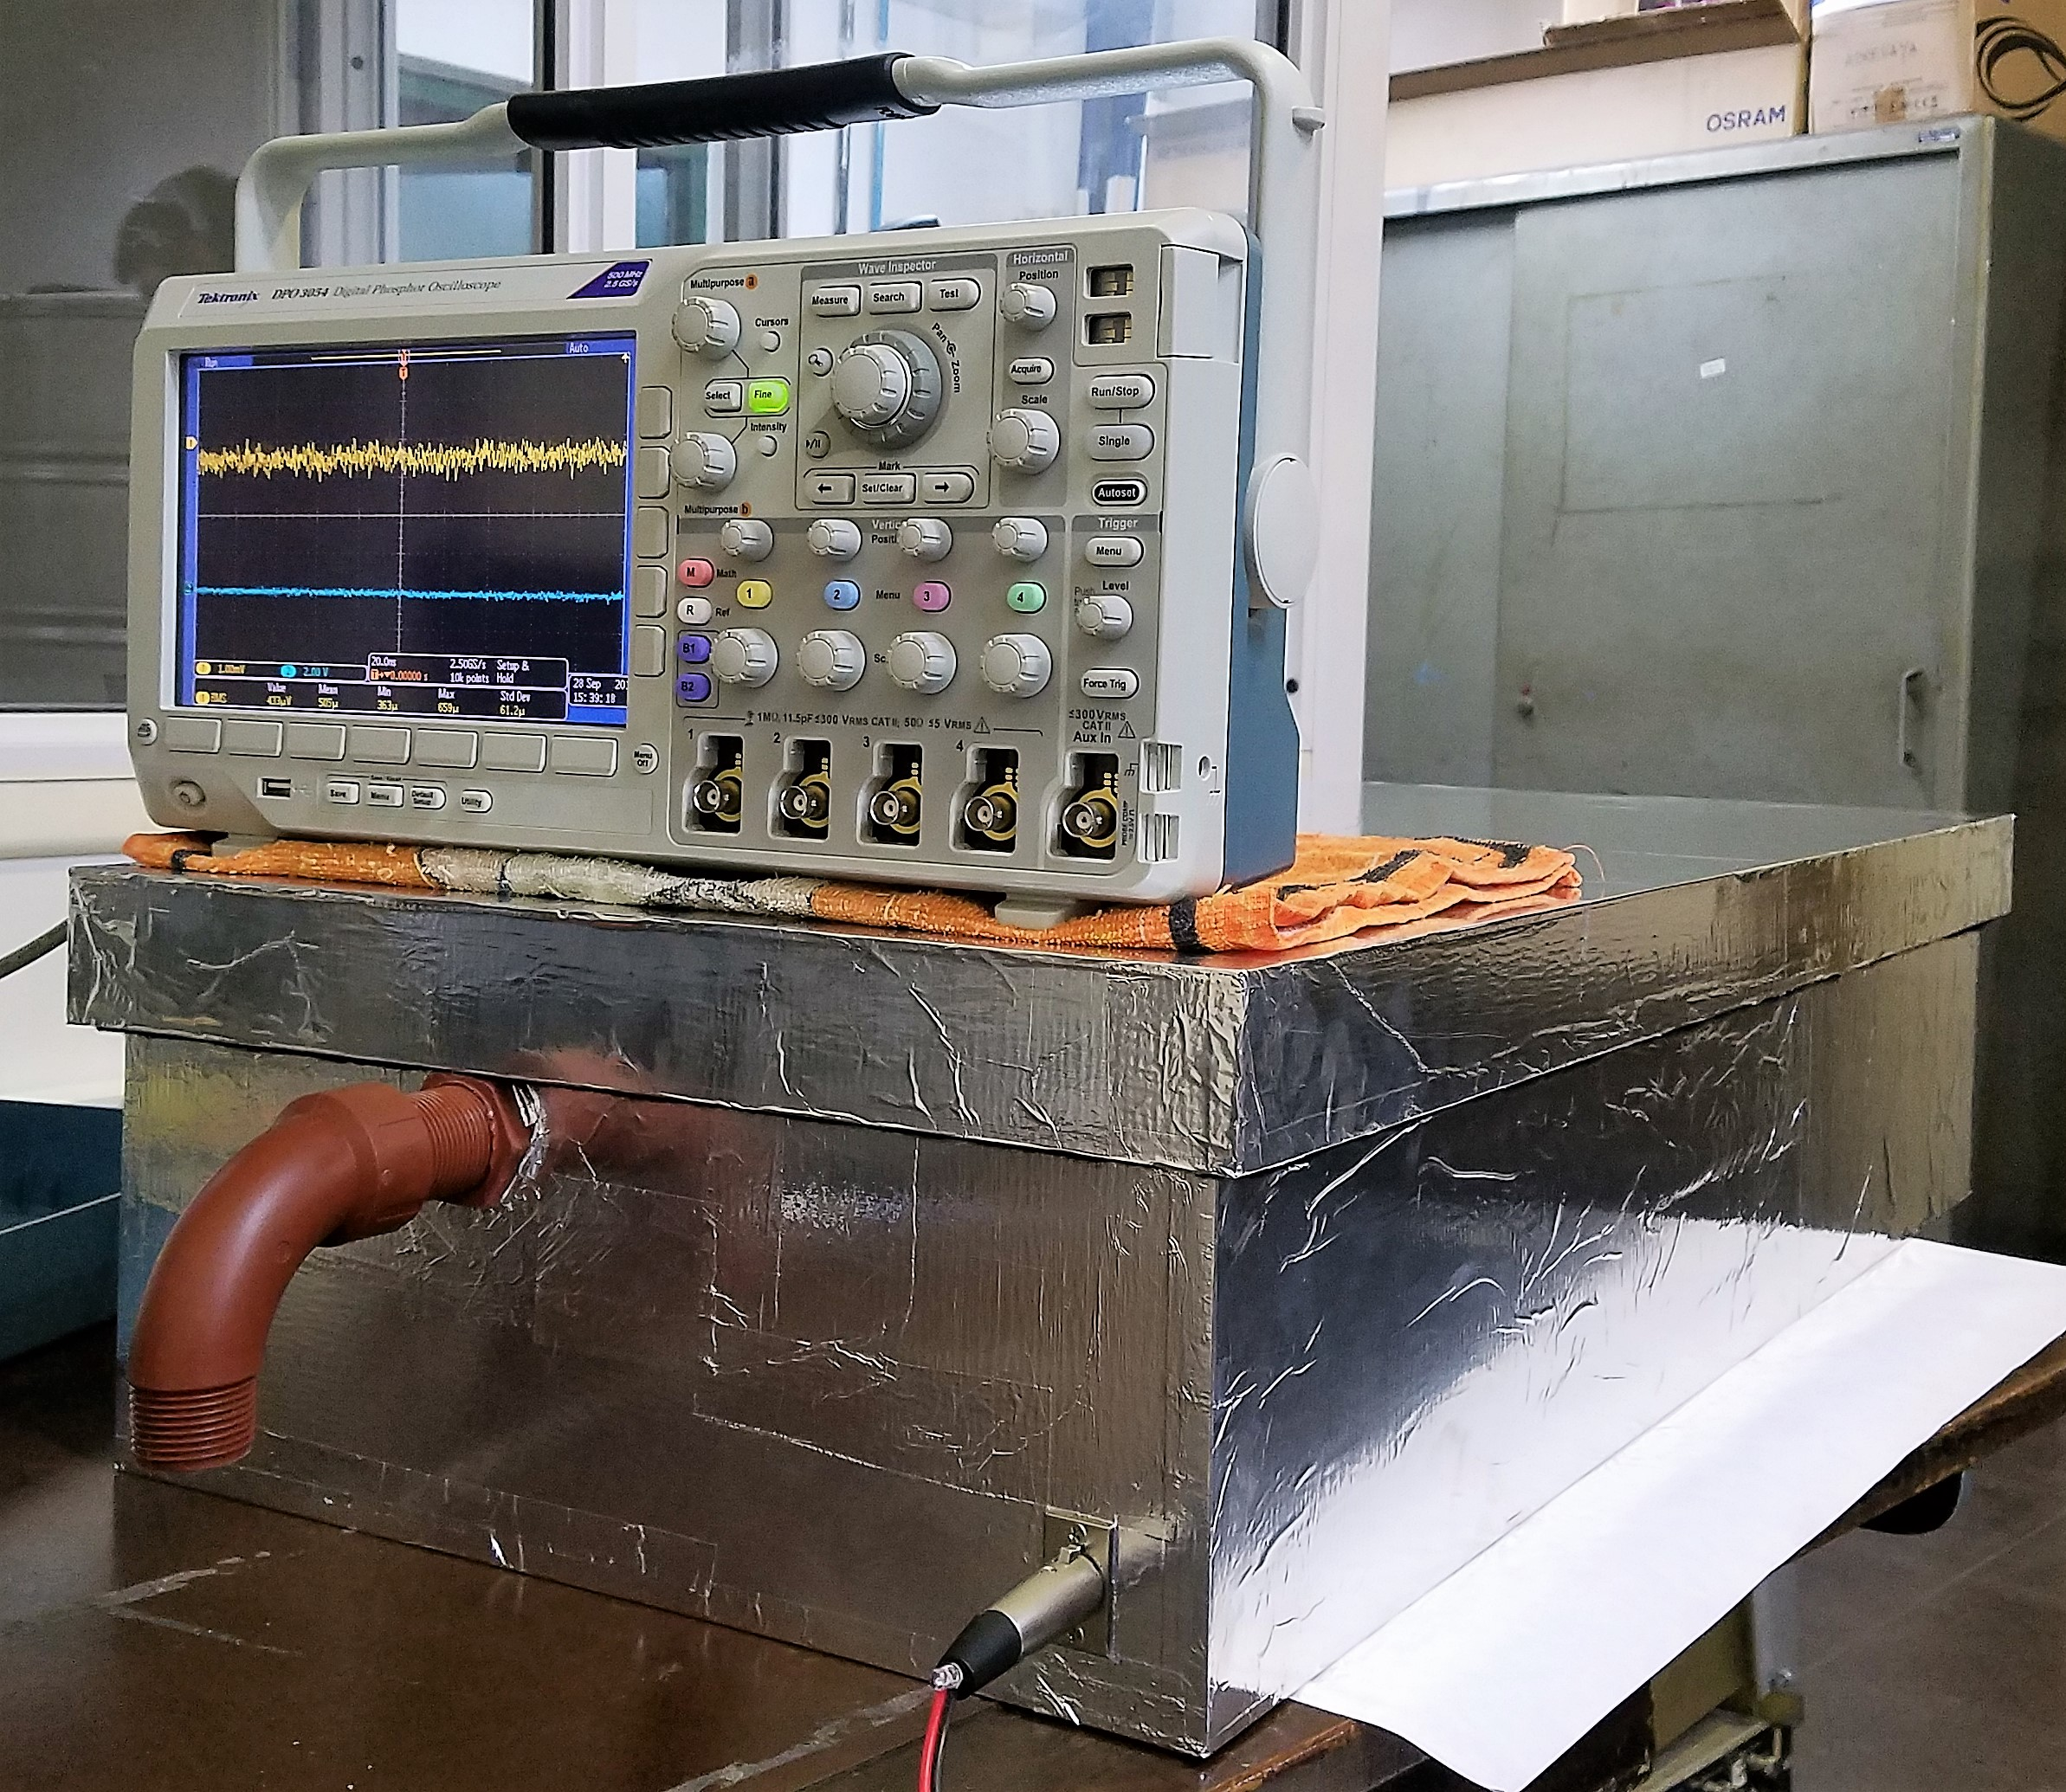
\includegraphics[width=.38\linewidth]{imgs/caja.jpg}
	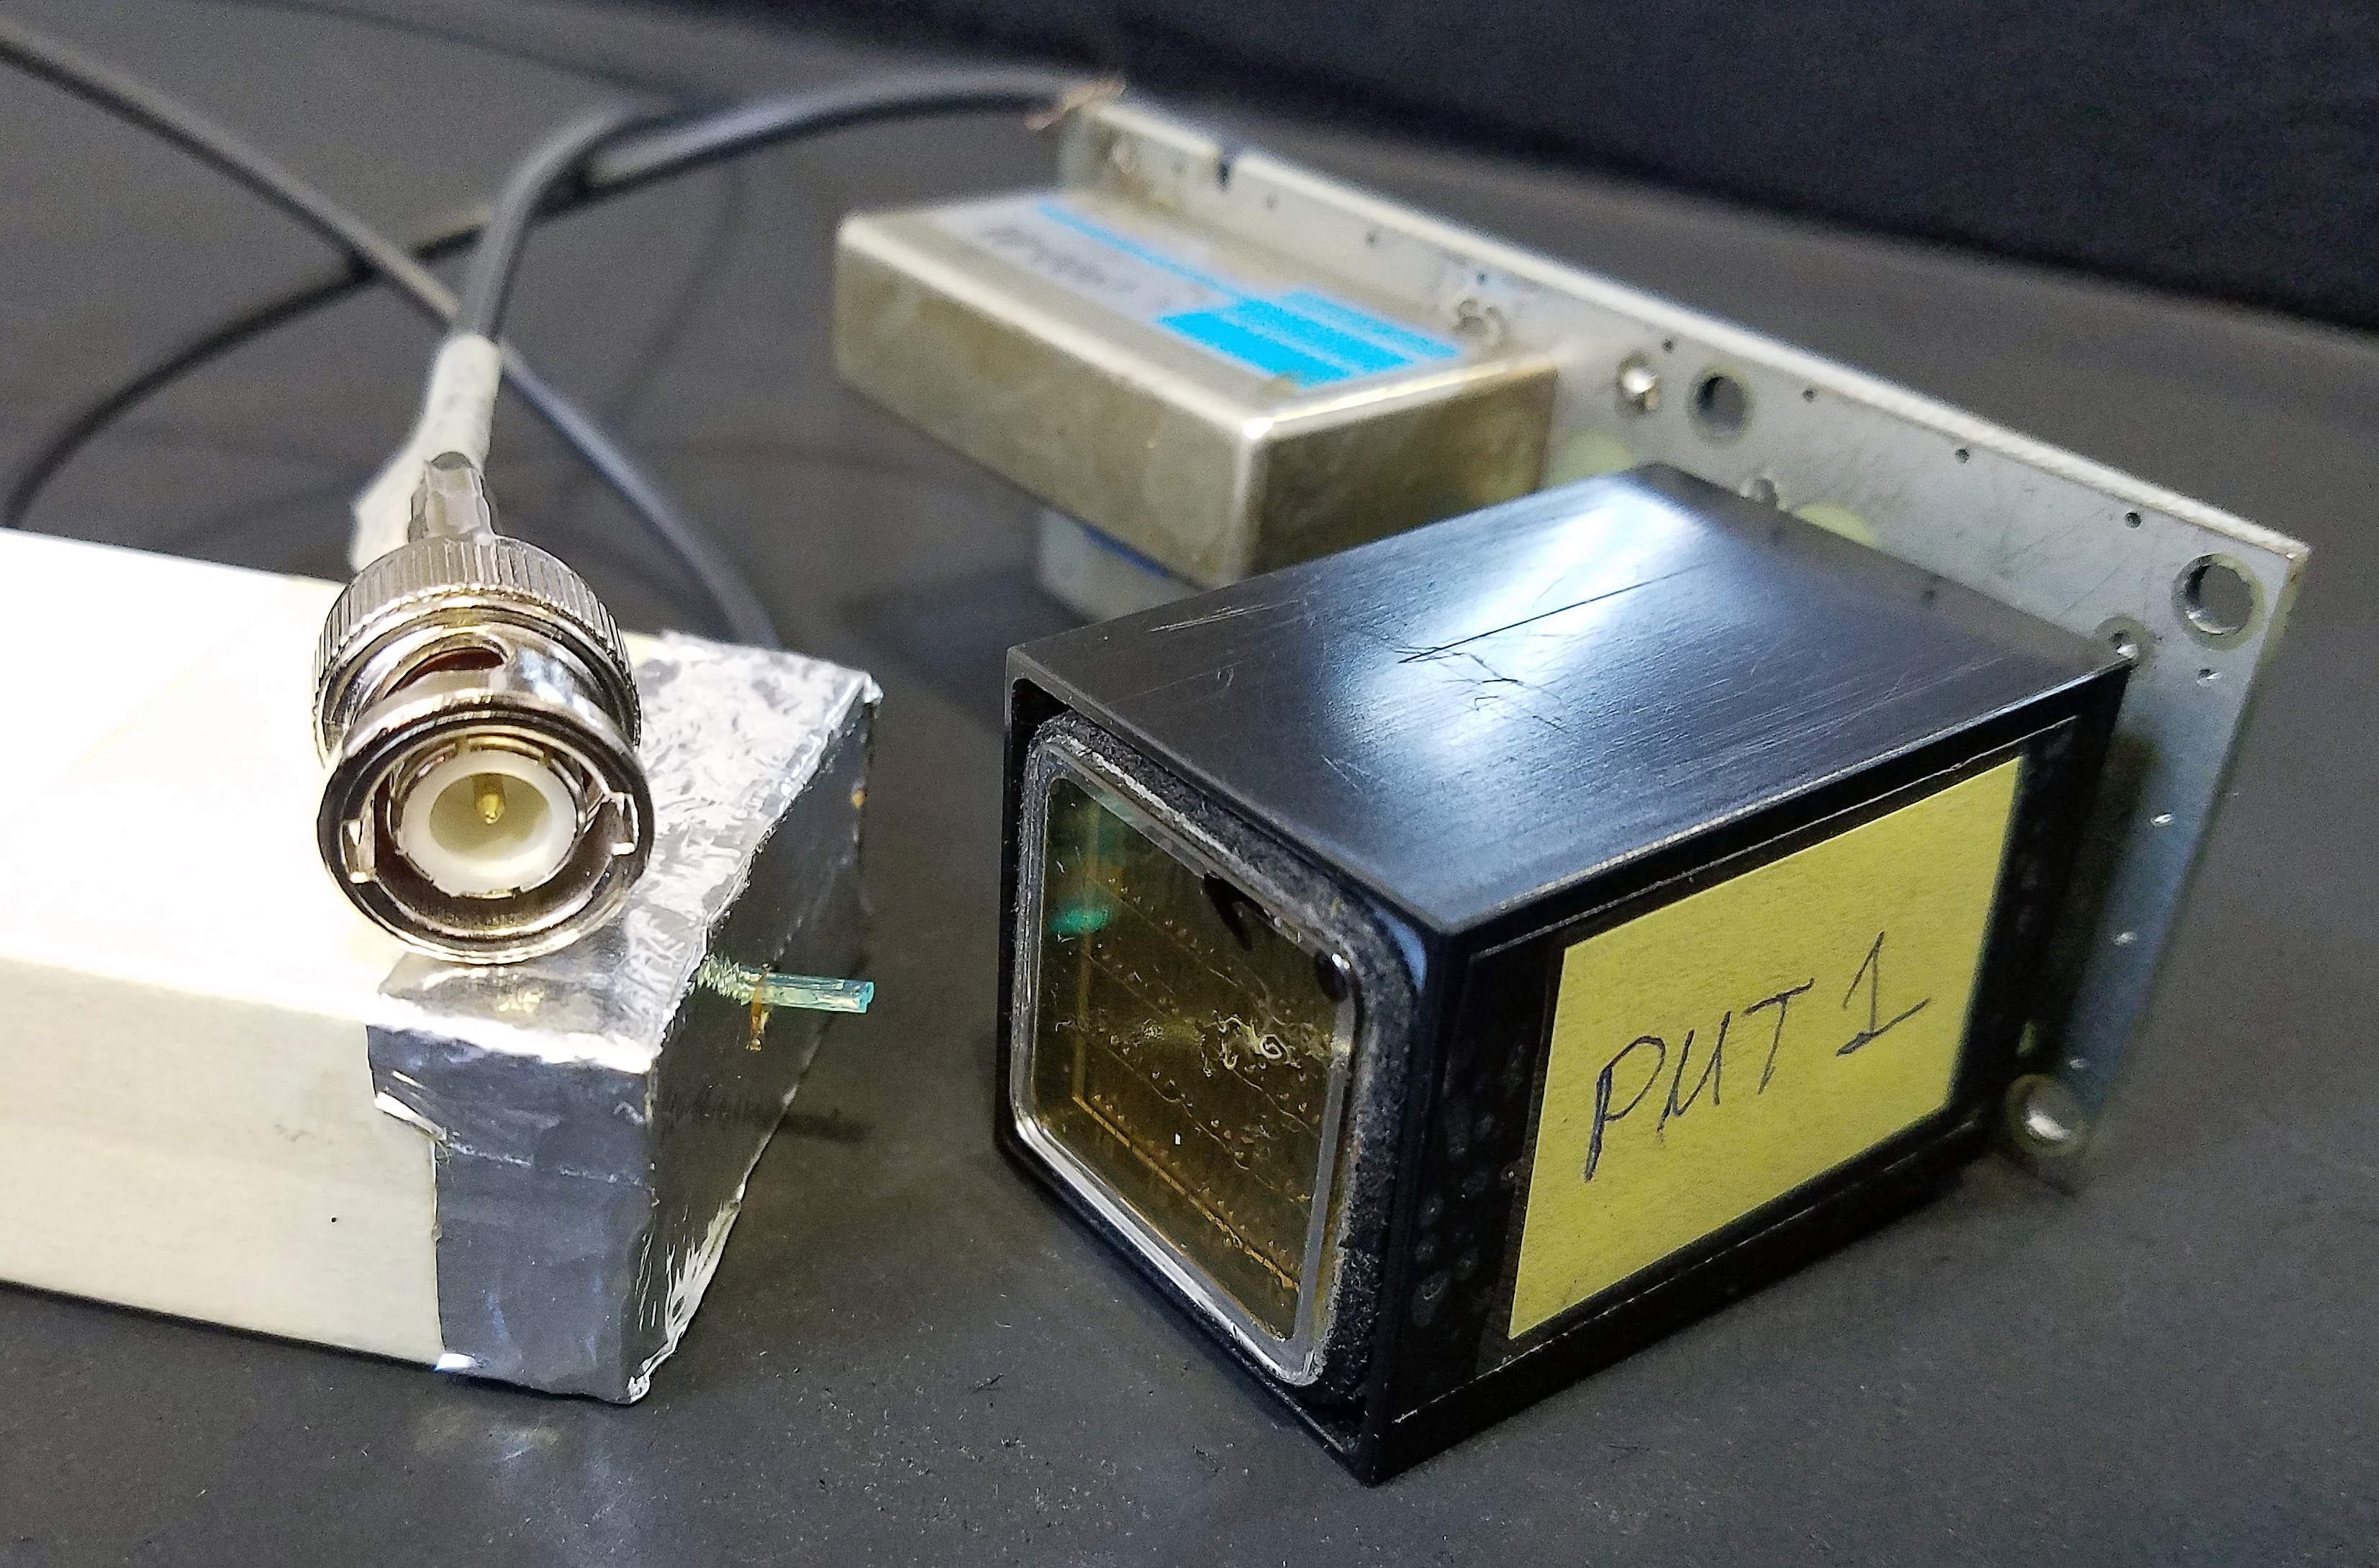
\includegraphics[width=.5\linewidth]{imgs/detector.jpg}
	\caption{Elementos básicos usados (no se muestra la tela blackout ni los muones).}
	\label{fig:setup}
\end{figure}

Para los detectores, se utilizaron placas centelladoras plásticas de $20\times4\text{ cm}^2$, con altura de $1$cm. Estas tenían una guía recortada a su largo por donde se colocaron dos fibras ópticas \textit{waveshifter} verdes que adecuaban la frecuencia de la señal al PMT. Para aumentar el tamaño de la señal se utilizaron dos placas para cada detector, ubicandolas una encima de la otra, con sus guías alineadas para formar una cavidad para las fibras. Con grasa óptica se apoyó la fibra sobre una de las 16 celdas fotocatódicas de los PMT Hamamatsu H8711-06, con pico de respuesta en $420$nm\cite{cacamatsu}. Estos recibían tensión de sus placas de alto voltaje Hamamatsu C4900, a su vez alimentadas con una fuente de 12V. Sobre esta misma placa se soldó un cable RG-174 para extraer la señal y medirla en un osciloscopio Tektronix DPO 3054. El setup completo puede observarse en la figura \ref{fig:setup}.

%Dado que se realizaron dos tipos de mediciones, uno correspondiente a la caracterización de los detectores por separado y otro la medición de coincidencias, Las posiciones de las placas variaron en uno u otro caso. Para las curvas de calibración (donde se midió el Rate de muones en función del voltaje de salida), la caja se ubicó con su lado mayor en forma horizontal y ambos detectores en distintas posiciones pero unidos por los cables de la fuente de $ 12V $. Por otro lado, para conincidencias se utilizaron dos configuraciones distintas. En la primera, se dejo la caja en la misma posición y se solaparon ambos centelladores uno sobre el otro. En la segunda, para variar la distancia entre centelladores, se utilizó la caja en forma vertical introduciendo un banco de madera fabricado en la tornería del IAFE para apoyar encima de él uno de los detectores, con esto se logró tener ambas placas distanciadas $ 50 cm $. Todo el circuito de la configuración horizontal y vertical puede apreciarse en la imagen XXX\\

%IMAGEN (a(horizontal) y b(vertical))\\

Se realizaron dos tipos de mediciones diferentes. Se caracterizó la salida de cada PMT individualmente registrando el número de pulsos con tensión mayor a cierto umbral, haciendo un barrido desde $1mV$ hasta $200mV$. El osciloscopio posee un contador interno que se incrementa cada vez que ocurre un disparo; variando el nivel del disparo y registrando número de eventos en cierto lapso de tiempo, se obtiene la frecuencia de pulsos de cada PMT en función del umbral. Esto fue realizado con el paquete pyvisa de Python. Una versión simplificada del código es el siguiente:

\small
\begin{verbatim}
rm = visa.ResourceManager('@py')
osci = rm.open_resource(rm.list_resources()[0],read_termination='\n')
muonesIniciales = int(osci.query('ACQuire:NUMACq?'))
time.sleep(60)
muonesNuevos = int(osci.query('ACQuire:NUMACq?')) - muonesIniciales
\end{verbatim}

\normalsize
Los fotocátodos de los PMT son propensos a la emisión termoiónica, por lo cual muchos de los pulsos de voltaje registrados no provienen de pulsos de luz enviados por el centellador. Por lo tanto, mediante el disparo \textit{Setup and Hold} de este osciloscopio, se realizaron mediciones de coincidencias. Este tipo de disparo ocurre cuando ambos canales superan un voltaje de referencia dentro de una ventana temporal. Para un muón energético viajando a una velocidad cercana a la de la luz, que son aquellos que sobreviven hasta llegar a nivel del mar, el tiempo que tarda en atravesar $4$cm de centellador será del orden de décimas de nanosegundo. Estos generaran una señal en prácticamente el mismo instante en ambos canales. Se puede establecer un elegir un voltaje distinto para cada canal de manera de asegurar que ambos PMT tengan la misma frecuencia de pulsos y minimizar las coincidencias casuales por efectos térmicos. De esta manera se puede obtener el número de eventos causados por muones, que en principio dependerá de la frecuencia de los PMT. 

\section{Resultados y discusiones}

%Previo a la calibración, el primer paso fue el estudio de los pulsos emitidos por los PMT's, sin placa centelladora. Esto nos dio una idea de la forma, amplitud y frecuencia de los pulsos provenientes del ruido de fondo. También se estudió la dependencia de estos parámetros con el alto voltaje y los pines, relación que resultó ser muy distinta para cada PMT. Para todas las mediciones se utilizaron los pines xxx y xxx con voltajes $ 852V $ y $ xxxV $ respectivamente, esta configuración daba amplitudes distintas para los pulsos de uno y otro PMT, aunque el ancho y espaciado temporal mínimo entre ellos \footnote{Esta frecuencia máxima corresponde a los pulsos de amplitudes menos negativas} resultó ser aproximadamente similar en ambos, siendo $ 6 ns $ y $ 160 ms $ respectivamente.

%Con estos análisis, se paso a introducir las placas centelladores para levantar las curvas de calibración. 
Los pulsos generados por estos PMT tienen un ancho que varía entre $10$ y $100$ns. El tamaño de los pulsos depende del voltaje de alimentación, pero no se caracterizó esta dependencia porque solo es modificable a partir de un potenciómetro sobre la placa de alta tensión, y se priorizó la búsqueda de coincidencias. Se optó por dejar los PMT en un voltaje fijo cercano a $1$kV, y para cada uno hacer un barrido de la frecuencia de pulsos en función del umbral establecido en el osciloscopio, entre $1$mV y $200$mV. Se observó que al dejar los PMT encerrados en oscuridad, disminuía la cantidad de pulsos pequeños de origen térmico, y que reaparecían al exponerlos a luz ambiente. Esto es usual; sin embargo, el proceso de enfriamiento fue más largo de lo esperado, ya que después de 14 días los PMT continuaban enfriándose, como puede verse en la figura comparativa \ref{fig:tengofrio}.
\begin{figure}[h]
	\centering
	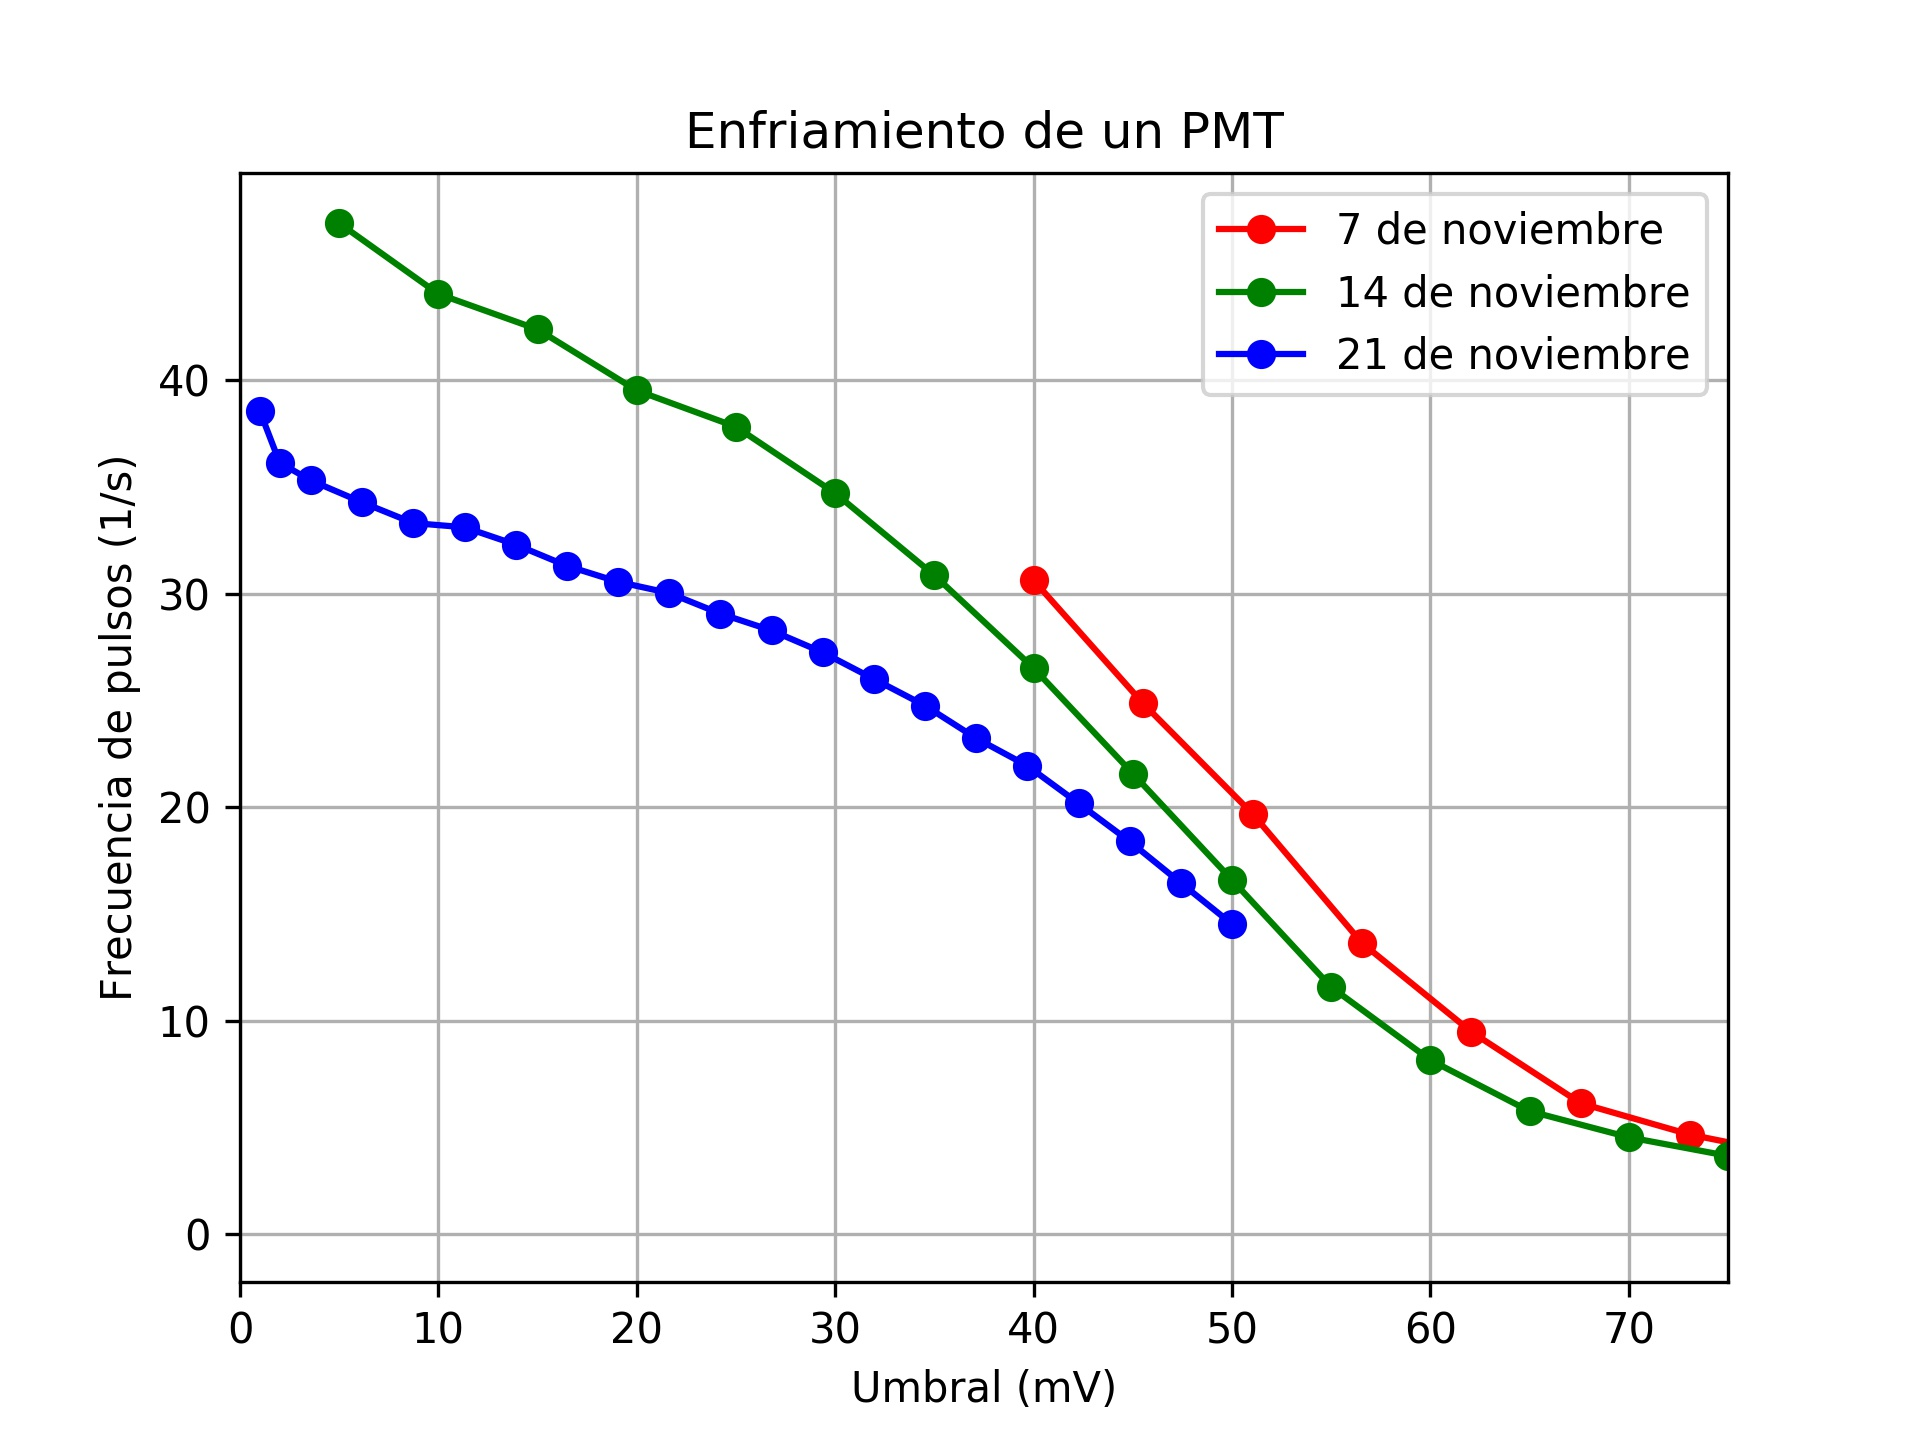
\includegraphics[width=.7\linewidth]{imgs/enfriamiento.jpg}
	\label{fig:tengofrio}
	\caption{Una selección de los barridos de un PMT que muestra la disminución con el tiempo de los pulsos más pequeños. Cada punto se midió a lo largo de una hora, en intervalos intercalados de diez minutos para asegurar un enfriamiento promedio parejo.}
\end{figure}

Esto dificulta saber qué frecuencia exacta tiene un PMT a un umbral dado, porque depende del día. Sin embargo, como los pulsos agregados son de origen térmico, no influyen sobre las coincidencias, como se muestra abajo. Usando una caracterización arbitraria, aquella en la cual los PMT tenían 7 días de oscuridad, y aprovechando la monotonía de las curvas, con un \textit{script} de Python se las invirtió. Esto permitió obtener los umbrales requeridos para lograr cierta frecuencia nominal, correspondiente a las condiciones de oscuridad mencionadas, pero no necesariamente representativas de las frecuencias de los PMT en otro momento. 

Para realizar la medición de coincidencias, se tomó en cuenta los tamaños de los pulsos y la máxima frecuencia de pulsos para el rango de voltajes analizado (aproximadamente $50$Hz, que implica, individualmente, $20$ms entre cada pulso). Se decidió retrasar uno de los canales en $17$ns, y se estableció una ventana temporal de $34$ns para observar coincidencias. Con esta configuración, se hicieron dos barridos de coincidencias en función de la frecuencia nominal de la caracterización escogida. Uno se lo hizo para PMT con varias semanas de oscuridad, y el otro para PMT recién expuestos a luz. La figura \ref{fig:tengocalor} muestra que el agregado de pulsos térmicos por luz ambiental no afecta las coincidencias, y que estas tienen una dependencia monótona creciente con la frecuencia de los PMT al tomar cortes por umbral. La independencia con el proceso de calentamiento y enfriamiento de los PMT indica que se trata de señales reales producidas simultáneamente en las barras centelladoras, provocadas por el paso de los muones.

\begin{figure}[h]
	\centering
	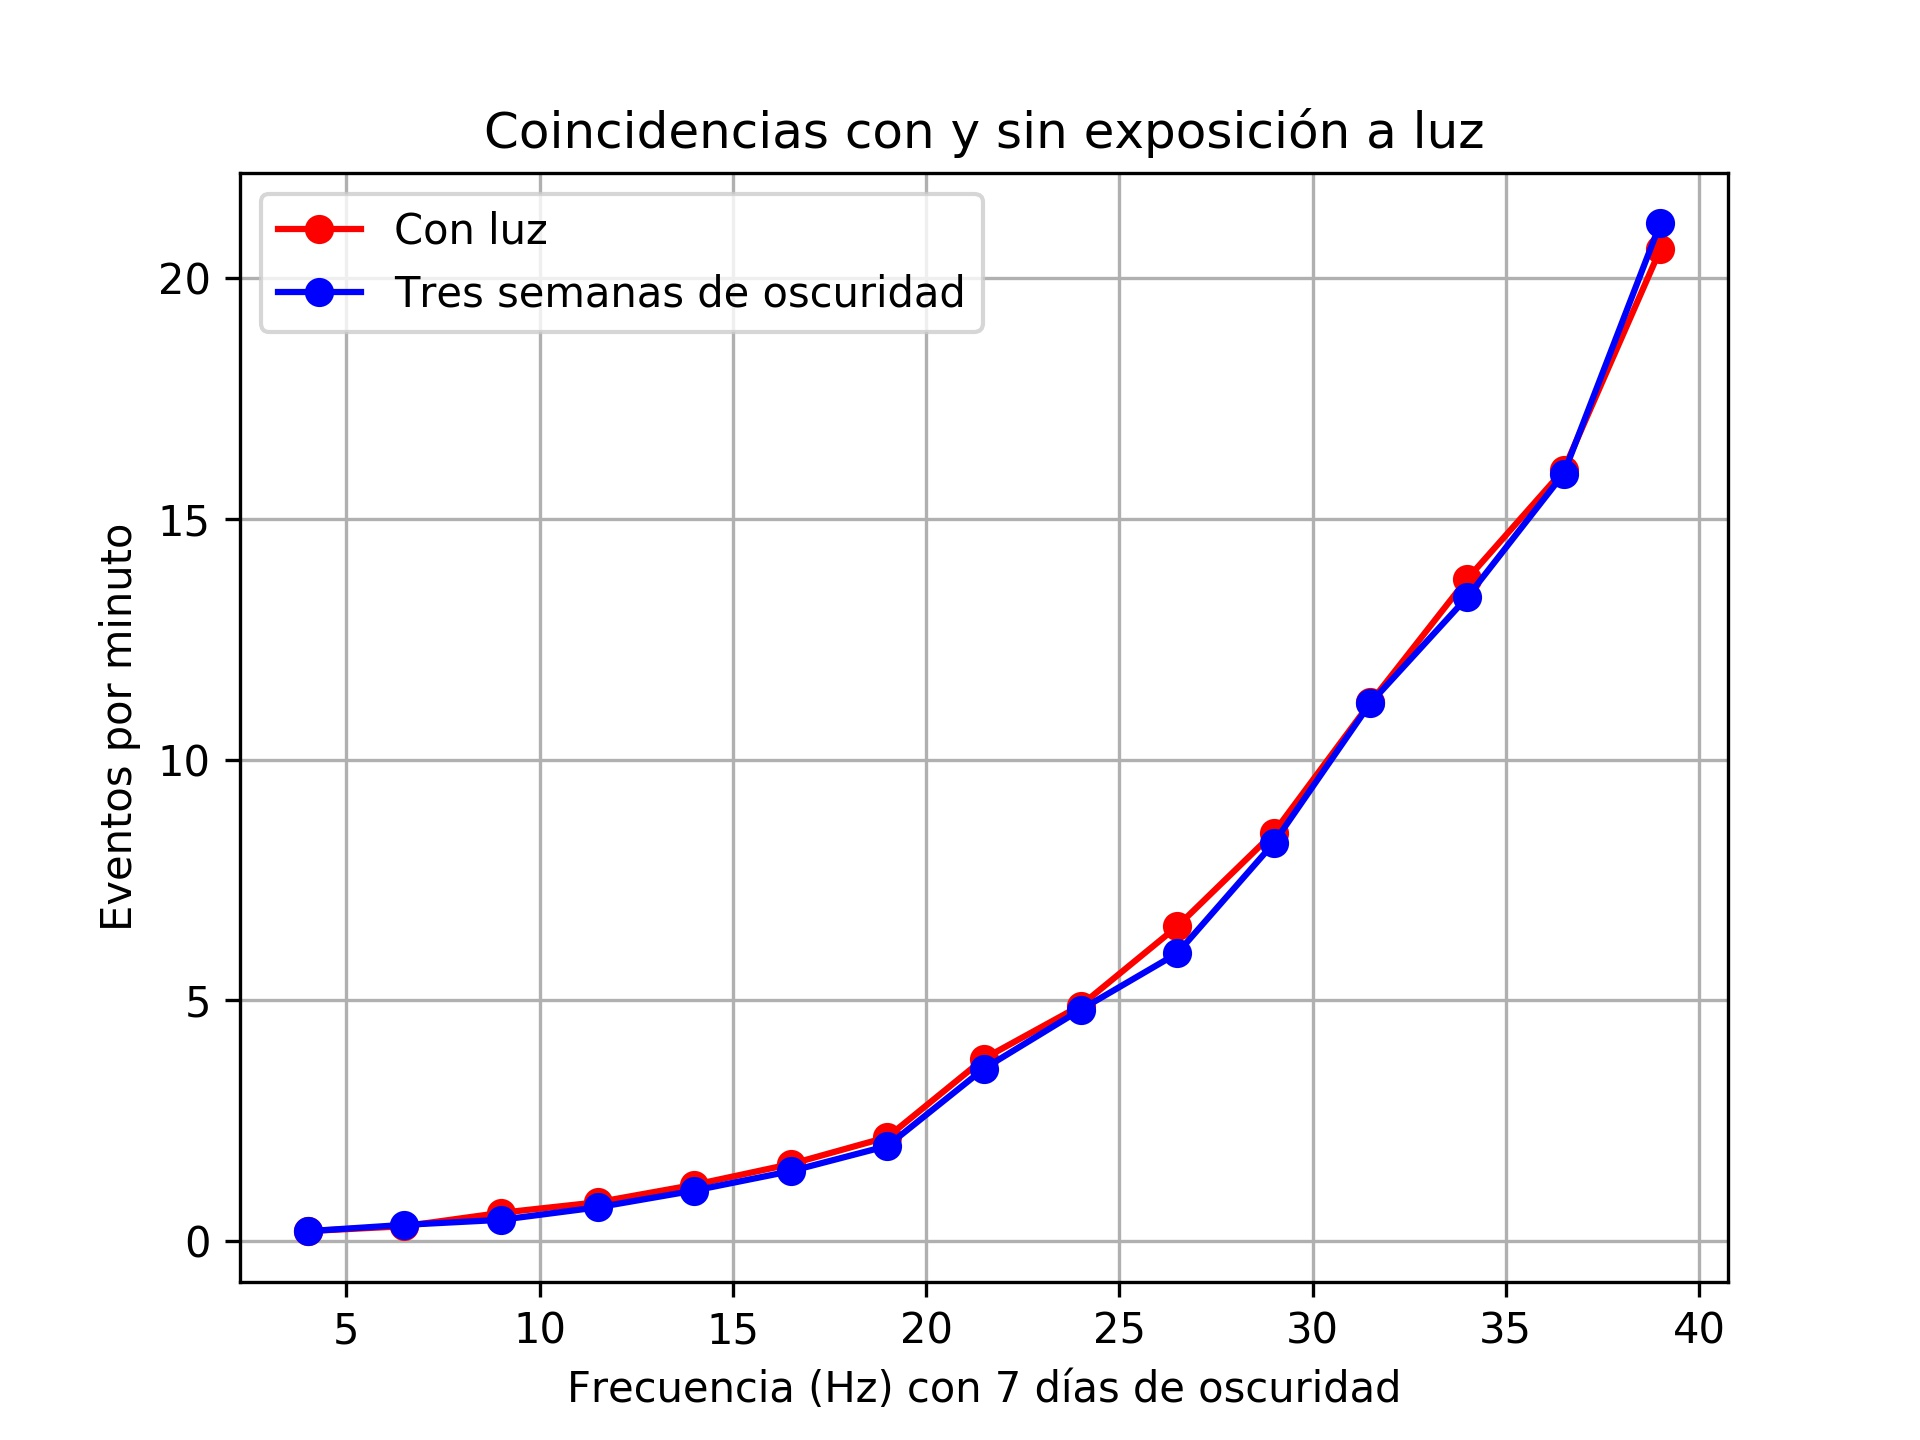
\includegraphics[width=.7\linewidth]{imgs/calentamiento.jpg}
	\label{fig:tengocalor}
	\caption{Una comparación de analizar coincidencias calentando los PMT con exposición a luz ambiental. El eje x se refiere a que se le dio a los PMT un umbral tal que, con 7 días de oscuridad, darían esa frecuencia.}
\end{figure}

La frecuencia máxima observada es de 20 eventos por minuto; pero dada la geometría del sistema, su área, y el flujo incidente de muones a nivel del mar (aproximadamente $0.007\text{cm}^{-1}\text{s}^{-1}\text{str}^{-1}\cos^2\theta$ donde $\theta$ es el ángulo polar), deberían observarse 52 eventos por minuto\cite{matematico_aleman}\cite{fisico_chino}, implicando una eficiencia del 38\%. Para corroborar esta medición, se separaron las placas $50$cm y se repitió la medición; se obtuvo una curva idéntica pero de menor amplitud. De los 3.5 eventos por minuto esperados, se observó un máximo de 1.1, una eficiencia similar del 31\%. Esto pareciera indicar un correcto funcionamiento, pero la geometría del detector y la caja limitan este tipo de mediciones, así como la baja precisión por el tamaño reducido de los centelladores. Con la elaboración de las paletas definitivas en Laboratorio 7, con movimiento independiente, se podrá relevar el flujo incidente de manera más precisa.

%Luego de las curvas de calibración y previo a la medición de coincidencias, se estudió la función Setup and Hold del osciloscopio, ya que jugó un papel clave en la medición de eventos. Para ello, se dedicó unos días a estudiar su funcionamiento simulando coincidencias con dos generadores de pulsos HP8013B y Rigol DG5101. Dicho estudio nos permitió ver la precisión y limitaciones de la ventana temporal así como los threshold mínimos y máximos permitidos.

%Al final creo que no hace falta lo de los pulsos

%Con esta información y utilizando el montaje de la figura xxx, se hizo un barrido de coincidencias entre placas en función de tasa de pulsos. Los resultados corresponden a la curva azul de la figura xxx. En ella, se consideraba una coincidencia si dos pulsos ocurrían distanciados en el tiempo por 17ns y superaban el threshold pedido: este threshold era calculado por el script de manera tal que ambos PMTs disparaban a una tasa conocida. Se eligió la ventana de $ 17 ns $ por la consideración de que los pulsos térmicos tenían un espaciado mínimo de $ 160 ms $ como se mencionó anteriormente, mientras que los muones viajando a una velocidad cercana a la de la luz, tardarían $ 0.1 ns $ en atravesar los $ 3 cm $ de grosor entre paletas. Si bien a este último tiempo se le debe agregar el retardo de emisión de los átomos dentro del centellador (del orden de ns) y la respuesta de la electrónica involucrada (PMT, cables,etc), todo esto no llega a ser comparable con el tiempo entre pulsos térmicos, por lo que dentro de esta ventana temporal caerán auténticos muones con un error dado por las \textbf{coincidencias casuales}. Estas últimas tiene una formula dada por\cite{coincidencias_casuales} (necesitamos esta referencia)
 
%\begin{equation}
%R_{casual}= 2 R_1 R_2 \tau
%\end{equation}

%donde $ R_1 $ y $ R_2 $ son la tasa de pulsos de cada detector y $ \tau $ la ventana temporal ($ 17 ns $). Si uno remplaza los valores de $ R_1 $ y $ R_2 $ máximos usados en las mediciones, puede verse que las coincidencias casuales rondan el $ 0.1 \% $, siendo despeciables para los eventos muónicos. Este número se buscó apropósito y es el responsable de haber utilizado xxx mv como Voltaje mínimo en la curva de calibración. Por otro lado, el porqué del máximo threshold es simplemente que no se registraban eventos más a allá de dicho valor.
%Luego, se repitió el experimento exponiendo los PMTs a luz para ver si el aumento de pulsos afectaría las coincidencias; la curva roja de la figura (?) indica que no.\\

%FIGURA(azul y roja)\\

%(capaz deberíamos meter un poco de discución acerca de la forma de la curva, la meseta y demás.)


%Para levantar esta segunda curva, si bien los PMTs estaban ''en caliente'' y disparando con un gran número de eventos, se usó la calibración de los PMTs con (?) días de oscuridad, en el sentido de que se establecieron thresholds que ya no se correspondían con la tasa de eventos reales que el PMT estaba midiendo, sino con la tasa que medirían tras (?) días. Esto se hizo bajo la suposición de que todos los eventos agregados serían de origen térmico y que entonces no contribuirían a las coincidencias, suposición que se vio corroborada.

%El último experimento constó de separar las placas y ver si el número de coincidencias disminuía. Efectivamente en la figura xxx se aprecia bla bla bla\\

%FIGURA\\

\section{Conclusiones}

Se construyó un entorno oscuro adecuado para realizar pruebas básicas sobre el funcionamiento del sistema de centelladores y fotomultiplicadores. Para estos últimos, se relevaron las características de la señal emitida a un voltaje fijo, y se observó un proceso prolongado de enfriamiento a lo largo de varias semanas. Sin embargo, se pudo establecer la independencia de la detección de coincidencias con el proceso de enfriamiento, indicando que las mediciones corresponden a pulsos generados simultáneamente en los centelladores por el paso de muones. Se estimó una eficiencia de entre el 30 y 40\% para el detector separando las barras centelladoras entre sí, dejando pendiente para el futuro una mayor caracterización del detector a partir de distribución conocida del flujo de muones.



\begin{thebibliography}{9}
	
	\bibitem{pierreauger}
	The Pierre Auger Collaboration, Proceedings 30 ICRC, arXiv:0710.1646
	
	\bibitem{cacamatsu}
	Hamamatsu Photomultiplier Tube Assembly H8711 Series\\
	https://www.hamamatsu.com/resources/pdf/etd/H8711\_TPMH1320E.pdf
	
	\bibitem{matematico_aleman}
	Mathar, R. 2015. Solid Angle of a Rectangular Plate. \\Max-Planck Institute of Astronomy.\\ http://www.mpia-hd.mpg.de/~mathar/public/mathar20051002.pdf 
	
	\bibitem{fisico_chino}
	Review of Particle Physics (28.3.Cosmic rays at the surface)\\
	K. A. Olive et al. (Particle Data Group), Chin. Phys C, 38, 090001(2014)
	
\end{thebibliography}

\section{Agradecimientos}

\begin{itemize}
	\item Pie de Tomás
	\item Codo de Adrián
	\item Muñeca de Gastón
\end{itemize}

\end{document}